%=========== ΛΥΣΗ ΘΕΜΑΤΟΣ Γ.94 ===========
\begin{thema}{Γ}

\begin{center}
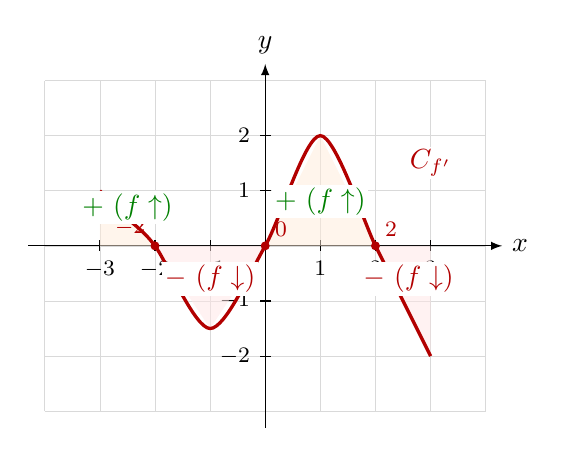
\begin{tikzpicture}[scale=0.7]
  \draw[help lines, gray!30] (-4,-3) grid (4,3);
  \draw[-latex] (-4.3,0) -- (4.3,0) node[right] {$x$};
  \draw[-latex] (0,-3.3) -- (0,3.3) node[above] {$y$};
  \foreach \x in {-3,-2,-1,1,2,3} \draw (\x,0.1) -- (\x,-0.1) node[below,font=\footnotesize] {$\x$};
  \foreach \y in {-2,-1,1,2} \draw (0.1,\y) -- (-0.1,\y) node[left,font=\footnotesize] {$\y$};
  
  \fill[orange!15, opacity=0.5, domain=-3:-2] (-3,0) -- plot coordinates {(-3,1) (-2.5,0.5) (-2,0)} -- cycle;
  \fill[red!10, opacity=0.5, domain=-2:0] (-2,0) -- plot coordinates {(-2,0) (-1,-1.5) (0,0)} -- cycle;
  \fill[orange!15, opacity=0.5, domain=0:2] (0,0) -- plot coordinates {(0,0) (1,2) (2,0)} -- cycle;
  \fill[red!10, opacity=0.5, domain=2:3] (2,0) -- plot coordinates {(2,0) (2.5,-1) (3,-2)} -- (3,0) -- cycle;
  
  \draw[very thick, red!70!black, smooth, tension=0.5]
    plot coordinates {(-3,1) (-2.5,0.5) (-2,0) (-1,-1.5) (0,0) (1,2) (2,0) (2.5,-1) (3,-2)};
    
  \filldraw[red!70!black] (-2,0) circle (2pt) node[above left,font=\footnotesize] {$-2$};
  \filldraw[red!70!black] (0,0) circle (2pt) node[above right,font=\footnotesize] {$0$};
  \filldraw[red!70!black] (2,0) circle (2pt) node[above right,font=\footnotesize] {$2$};
  \node[red!70!black, fill=white, inner sep=1pt] at (3,1.5) {$C_{f'}$};
  
  % Monotonicity signs for f
  \node[green!50!black, fill=white, inner sep=1pt] at (-2.5, 0.7) {$+$ ($f \uparrow$)};
  \node[red!70!black, fill=white, inner sep=1pt] at (-1, -0.6) {$-$ ($f \downarrow$)};
  \node[green!50!black, fill=white, inner sep=1pt] at (1, 0.8) {$+$ ($f \uparrow$)};
  \node[red!70!black, fill=white, inner sep=1pt] at (2.6, -0.6) {$-$ ($f \downarrow$)};
\end{tikzpicture}
\end{center}

\begin{erwthma}

\item \textbf{Μονοτονία και Ακρότατα (Μέσω Πίνακα Μεταβολών):}
Διατηρώντας στο νου ότι το σχήμα αναπαριστά την $\mathbf{f'(x)}$ (παράγωγο), το ενδιαφέρον μας στρέφεται αποκλειστικά στο \textbf{πρόσημό της} (που αφορά το πάνω/κάτω από τον άξονα των $x$).
- Περιοχή $[-3, -2)$ : Η $C_{f'}$ είναι πάνω από τον άξονα $\Rightarrow f'(x) > 0 \Rightarrow \mathbf{f \uparrow}$. 
- Περιοχή $(-2, 0)$ : Η $C_{f'}$ είναι κάτω από τον άξονα $\Rightarrow f'(x) < 0 \Rightarrow \mathbf{f \downarrow}$.
- Περιοχή $(0, 2)$ : Η $C_{f'}$ είναι πάνω από τον άξονα $\Rightarrow f'(x) > 0 \Rightarrow \mathbf{f \uparrow}$.
- Περιοχή $(2, 3]$ : Η $C_{f'}$ είναι κάτω από τον άξονα $\Rightarrow f'(x) < 0 \Rightarrow \mathbf{f \downarrow}$.

Με βάση τον Πίνακα Προσήμων - Μεταβολών, αντλούμε τα ακρότατα της $f$:
- Στο $\mathbf{x = -3}$ : Τοπικό \textbf{Ελάχιστο} (ακρότατο αριστερού άκρου ανόδου).
- Στο $\mathbf{x = -2}$ : Τοπικό \textbf{Μέγιστο} (εναλλαγή από $\uparrow$ σε $\downarrow$).
- Στο $\mathbf{x = 0}$ : Τοπικό \textbf{Ελάχιστο} (εναλλαγή από $\downarrow$ σε $\uparrow$).
- Στο $\mathbf{x = 2}$ : Τοπικό \textbf{Μέγιστο} (εναλλαγή από $\uparrow$ σε $\downarrow$).
- Στο $\mathbf{x = 3}$ : Τοπικό \textbf{Ελάχιστο} (ακρότατο δεξιού άκρου καθόδου).

\item \textbf{Σημεία Καμπής της $f$:}
Τα σημεία καμπής της αρχικής συνάρτησης συμβαίνουν εκεί που η παράγωγός της ($f'$) αλλάζει μονοτονία (δηλαδή παρουσιάζει τοπικά ακρότατα).
Παρατηρώντας το γράφημα της $f'$:
1. Στην περιοχή $-1$, η άνοδος της $f'$ σταματά σε κοιλιά $\Rightarrow$ παρουσιάζει \textbf{ελάχιστο} (άρα πρώτη καμπή).
2. Στη θέση $1$, η άνοδος σταματά σε κορυφή $\Rightarrow$ παρουσιάζει \textbf{μέγιστο} (δεύτερη καμπή).
3. Στη θέση $2{,}5$, καταχωρείται \textbf{ελάχιστο} (τρίτη καμπή).
Η $C_f$ παρουσιάζει, συνεπώς, \textbf{τρία (3) σημεία καμπής} γύρω από τις κεντρικές θέσεις $x_1 \approx -1$, $x_2 \approx 1$ και $x_3 \approx 2{,}5$.

\item \textbf{Θεώρημα Μέσης Τιμής στο $[-2, 2]$:}
Η συνάρτηση $f$ ικανοποιεί τις συνθήκες του ΘΜΤ (καθώς παρουσιάζει συνεχή παράγωγο). Συνεπώς, υπάρχει $\xi \in (-2, 2)$ τέτοιο ώστε:
\[ f'(\xi) = \frac{f(2) - f(-2)}{2 - (-2)} \Rightarrow \mathbf{f'(\xi) = \frac{f(2) - f(-2)}{4}} \]
(Αυτό είναι το γενικό ζητούμενο αν δεν προσδιορίζεται η ακριβής υλοποίηση του εμβαδού από το γράφημα).

\item \textbf{Εφαρμογή του Θεωρήματος \eng{Rolle} και πλήθος ριζών:}
Εάν δοθεί $f(-2) = 3$ και $f(2) = 3$, δημιουργείται η περιζήτητη ισότητα στα άκρα. Η $f$ συνεχής στο $[-2, 2]$ και παραγωγίσιμη, οπότε ικανοποιεί τις προϋποθέσεις του Θεωρήματος \eng{Rolle}.
Επομένως, \textbf{υπάρχει τουλάχιστον μία} ρίζα $\xi \in (-2, 2)$ της παραγώγου εξίσωσης $f'(\xi) = 0$.

\textbf{Πόσες ρίζες βρίσκουμε γραφικά:} Κοιτάζοντας το γράφημα της $f'$ εντός του διαστήματος $(-2, 2)$ (δηλαδή τα σημεία που τέμνει τον οριζόντιο άξονα), διαπιστώνουμε ότι η μοναδική «ρίζα» είναι το σημείο \textbf{$\boldsymbol{x = 0}$}. Άρα εντοπίζουμε **ακριβώς 1 ρίζα** της παραγώγου εξίσωσης στο εν λόγω ανοιχτό διάστημα.

*(Σημείωση: Αν η ερώτηση αφορούσε τις ρίζες της **ίδιας της συνάρτησης** $f(x)=0$: η $f$ κατέρχεται από $f(-2)=3$ έως $f(0)=1$ και ξανανεβαίνει στο $f(2)=3$. Μη έχοντας λάβει ποτέ αρνητικές τιμές ή αγγίξει το $0$, η εξίσωση $f(x)=0$ θα είχε $\mathbf{0}$ ρίζες).*
\end{erwthma}
\end{thema}
